% copyright 2020 Edmundo Carmona Antoranz
% Released under the terms of Creative Commons Attribution-ShareAlike 4.0 International Public License

\section{Full file conflicts}

So, have you enjoyed all the previous conflicts? I bet you have. Well... if you liked those, you will {\bf love} this one!

\subsection{Example 17}

From \hyperref[openjdk_repo]{OpenJDK's JDK repo}, checkout revision {\bf 9d3e0870754} and merge {\bf 2978ffb9f9d}\footnote{these are
the parents of revision {\bf e005d5df51e}}.

You will see a conflict pop up on file {\bf langtools/src/share/classes/com/sun/tools/doclets/internal/toolkit/resources/doclet.xml}.
But it is not just {\it a} conflict. It is {\bf the} conflict. Instead of having a few conflicted lines, the whole file is conflicted.
Here are some excerpts from it (line numbers are visible on the left side):

\begin{lstlisting}[style=console_style,
	basicstyle=\small,
	caption={\bf example 17} - conflicted file]
     1  <<<<<<< HEAD
     2  <?xml version='1.0' encoding='utf-8'?>
     3  
     4  <!--
     5   Copyright 2003 Sun Microsystems, Inc.  All Rights Reserved.
.
.
.
   205      </SerializedForm>
   206  </Doclet>
   207  ||||||| 4ae52d7dc1e
   208  <?xml version='1.0' encoding='utf-8'?>
   209  
.
.
.
   411      </SerializedForm>
   412  </Doclet>
   413  =======
   414  <?xml version='1.0' encoding='utf-8'?>
   415  
   416  <!--
.
.
.
   616          <Footer/>
   617      </SerializedForm>
   618  </Doclet>
   619  >>>>>>> 2978ffb9f9d
\end{lstlisting}

Before I go into the details, let me show you what happened in {\bf the other branch} in terms of changes for this file:

\begin{lstlisting}[style=console_style,
	basicstyle=\small,
	caption={\bf example 17} - changes from {\bf the other branch}]
$ git diff HEAD...MERGE_HEAD -- langtools/src/share/classes/com/sun/tools/doclets/internal/toolkit/resources/doclet.xml
diff --git a/langtools/src/share/classes/com/sun/tools/doclets/internal/toolkit/resources/doclet.xml b/langtools/src/share/classes/com/sun/tools/doclets/internal/toolkit/resources/doclet.xml
index 8eaa2d77abc..29c473790e4 100644
--- a/langtools/src/share/classes/com/sun/tools/doclets/internal/toolkit/resources/doclet.xml
+++ b/langtools/src/share/classes/com/sun/tools/doclets/internal/toolkit/resources/doclet.xml
@@ -1,7 +1,7 @@
 <?xml version='1.0' encoding='utf-8'?>
 
 <!--
- Copyright 2003 Sun Microsystems, Inc.  All Rights Reserved.
+ Copyright 2003-2009 Sun Microsystems, Inc.  All Rights Reserved.^M
  DO NOT ALTER OR REMOVE COPYRIGHT NOTICES OR THIS FILE HEADER.
 
  This code is free software; you can redistribute it and/or modify it
\end{lstlisting}

A simple one-liner of a change. Is the line different from what we have in {\bf HEAD}?

\begin{lstlisting}[style=console_style,
	basicstyle=\small,
	caption={\bf example 17} - file as it is on {\bf HEAD}]
$ git show HEAD:langtools/src/share/classes/com/sun/tools/doclets/internal/toolkit/resources/doclet.xml | head -n 5
<?xml version='1.0' encoding='utf-8'?>

<!--
 Copyright 2003 Sun Microsystems, Inc.  All Rights Reserved.
 DO NOT ALTER OR REMOVE COPYRIGHT NOTICES OR THIS FILE HEADER.
\end{lstlisting}

The line looks exactly like what is removed on {\bf the other branch}... this looks like a no-brainer, right? There should be {\bf no
conflict, whatsoever}. What happened then? There's a short-answer to this question but.... how will I spare us the pleasure of a
long-story?

Text files are made up of {\bf lines}. git considers the separate lines that make up a file to see {\it which lines} are the same
and which lines have changed in order to merge code. Now, have you ever asked yourself how {\bf a line} is defined? Each line is
separated from the next by a marker called {\bf End Of Line} (or {\bf EOL}, for short). But there is a tiny little problem: there are
not one or two but {\bf three}(!!!) different EOL markers and each one is associated with a different operating system.

\begin{itemize}
	\item {\bf Mac}: {\bf CR} ({\bf Carriage Return}, char {\bf 0x0d}, what we normally treat as {\bf {\textbackslash}r} in programming languages)
	\item {\bf NIX}: {\bf LF} ({\bf Line Feed}, char {\bf 0x0a}, what we normally treat as {\bf {\textbackslash}n} in programming languages)
	\item {\bf Windows}: {\bf CRLF} ({\bf Carriage Return} followed by {\bf Line Feed}, chars {\bf 0x0d0a})
\end{itemize}

Here's a little text file with different EOL formats so you can see the difference at the binary level:
\begin{figure}
	\centering
	\caption{{\bf Mac} EOL}
	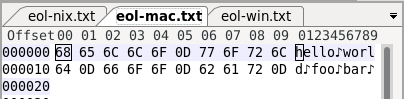
\includegraphics{eol-mac.png}
	\caption{{\bf NIX} EOL}
	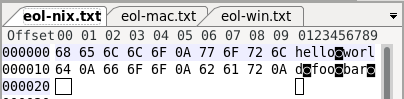
\includegraphics{eol-nix.png}
	\caption{{\bf Windows} EOL}
	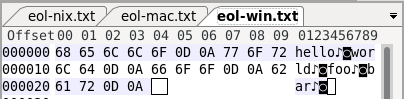
\includegraphics{eol-win.png}
\end{figure}

On a new file, text editors tend to set the EOL format to the one associated with the Operating System that the editor is running on.
If the file already existed, text editors\footnote{At least, {\it decent} text editors} will keep using the format that the file had
when it was opened, even if it is different from the OS that the editor is running on. Go save a text file with different EOL formats
and open it on a hex editor and see how the markers between the lines change.

You might be asking yourselves ``How did we end up in this EOL mess?'' It's a fair question to ask and, just like any other good story,
it's about betrayals, backstabbings from close friends and greed but it's way outside of the focus of this manual so I will kindly ask you to
read \href{https://en.wikipedia.org/wiki/Newline#History}{Wikipedia's Newline History} if you are curious to know how this mess came
to be.

Coming back to our problem at hand, from the point of view of git, a change in EOL format will effectively change the content of
{\bf each and every single line} that makes up the file. So, you open a preexisting file, you change a single line and then save using
the wrong EOL format, and to git it's like the whole file was cleared up and rewritten as a whole... in Esperanto. It's an entirely
different content from top to bottom. Let me say it again, just so that the concept sinks in: {\bf Completely (dramatic pause) Different
(dramatic pause) File}. None of the preexisting lines survived that revision.

Now, is that {\bf really} the case of what happened over here? Well, let's get the info from {\bf unix2dos} to see how many
{\bf line-breaks} of each type there are:

\begin{lstlisting}[style=console_style,
	basicstyle=\small,
	caption={\bf example 17} - file types]
$ git show HEAD:langtools/src/share/classes/com/sun/tools/doclets/internal/toolkit/resources/doclet.xml | unix2dos -imud
       0     205       0
$ git show MERGE_HEAD:langtools/src/share/classes/com/sun/tools/doclets/internal/toolkit/resources/doclet.xml | unix2dos -imud
     205       0       0
$ git show 4ae52d7dc1ef:langtools/src/share/classes/com/sun/tools/doclets/internal/toolkit/resources/doclet.xml | unix2dos -imud
     205       0       0
\end{lstlisting}

And we can see how on {\bf HEAD} the line breaks are on a different column, which indicates a change of {\bf EOL format}.

Before considering what to do about it, let us ask ourselves ``{\bf why did this happen in the first place?}'' To our own amazement,
there are some rather simple possibilities for this to come up:

\begin{itemize}
	\item {\bf Developer changed it on purpose}. There might be a technical reason for that (Hard to come up with one but...).
	But if it was just for the sake of it, this deserves a call of attention because of the burden downstream that it creates
	(you will see).
	
	\item {\bf Editor (IDE, text editor) changed it} without the Developer being aware of it. Hey, it happens! Have you ever opened
	a NIX file in Window's notepad? Saved the file without thinking about it? There you go!
	\footnote{When you open the file, it will look like a very long single line because notepad will fail to recognize the {\bf LF}
	chars as line breaks. It has to be {\bf CRLF} because {\it who in their right mind would use something other than Microsoft software
	in the first place}, right? Therefore, when you save the file (if you fail to realize what happened when you opened the file and
	didn't run away from it), all line breaks will be gone. And if you decided to go separating the lines one by one in notepad and
	save them (Hey! Not all developers are in a rush to do stuff, you know?), then all the lines have been changed to have
	{\bf CRLF} line breaks instead of the original {\bf LFs}. And if this criticism is not true {\it anymore} because a new Microsoft
	Notepad has come out that supports different EOL formats, then let me say {\it “Great!”} Too bad it is coming some 30+ years too
	late. So I stand behind my criticism.}
	And I bet there are other editors out there that don't keep the original EOL format {\bf at all}. Either way, this should have been
	caught by the developer {\bf before} publishing the changes for other people to pull because if another developer changes the file
	and then pulls (merges/rebases/cherry-picks) the change where the other developer changed the EOL, they end up with a nasty
	full-length conflict like the one we are talking about... {\bf even if the revisions are related to single-line changes}. If you use
	a decent git front-end to see what a revision looks like, you would see that even if you meant to change a few lines from the
	file, the whole file will show up as being cleared up and then added back, from top to bottom. That's the tell-tale symptom
	that should make you realize that there is a problem and you should correct it {\bf before publishing it}.
	
	\item {\bf git itself is getting in the way}. git has a few tricks that can be used to set EOL format of files. Personally,
	I find them extremely difficult to set up correctly, specially considering developers using different operating systems,
	IDEs, etc. I always recommend to set up git to not care about EOL formats and let developers take care of them. And this can
	be done with a small setting in {\bf .gitattributes} so that it can be shared by whoever works on the project. And if you are
	certain that you want to have git take care of EOL format, then make sure to read all the details about it starting with
	{\bf git help attributes}, specifically the section related to {\bf checking-out} and {\bf checking-in}. That will do for a really
	nice read. Last but not least, do not fall for the {\bf core.autocrlf} trap. Read what is is about {\bf before} deciding what
	value you should use for that\footnote{If you use the wrong value for that on the global config, you will easily mess up many of
	the files of the project {\it without even opening a single one}.}.
	
\end{itemize}

Ok, ok... enough theory. Let's consider the different approaches you might follow to get out of this mess.

\subsection*{Stay on HEAD, bring over changes from the other branch}

First thing to notice is that this is kind of offsetting the purpose of the merge, right? You would like to get all changes from
{\bf the other branch} {\it automagically} copied over on your code {\bf and} get conflicts on the pieces that are rightly so.
Now we are in a situation where we will need to do everything {\bf by hand}. Luckily for us, in this case, we have already seen what is
required to bring over from {\bf the other branch}. We need to adjust the years covered in the copyright. So, this would be the
resulting file, the first few lines:

\begin{lstlisting}[style=xml_style,
	basicstyle=\small,
	caption={\bf example 17} - {\bf HEAD} with changes from {\bf the other branch}]
<<<<<<< HEAD
<?xml version='1.0' encoding='utf-8'?>

<!--
 Copyright 2003-2009 Sun Microsystems, Inc.  All Rights Reserved.
 DO NOT ALTER OR REMOVE COPYRIGHT NOTICES OR THIS FILE HEADER.
\end{lstlisting}

Then we remove the other parts and the conflict markers. Then wrap up the merge:

\begin{lstlisting}[style=console_style,
	basicstyle=\small,
	caption={\bf example 17} - Wrap up the merge]
$ git add langtools/src/share/classes/com/sun/tools/doclets/internal/toolkit/resources/doclet.xml
$ git merge --continue
[detached HEAD b4a035c194c] Merge commit '2978ffb9f9d' into HEAD
\end{lstlisting}

That's good. As as a quick fix, this does the job... {\bf but} you haven't really tackled the {\bf root cause of the problem}.
There is still an {\bf EOL-format} discrepancy between the branches. As a little experiment, let's checkout the revision
we just asked to merge, {\bf 2978ffb9f9d}, let's write a little change on this file and then let's come back to the merge
revision we just created and ask to merge again.

\begin{lstlisting}[style=console_style,
	basicstyle=\small,
	caption={\bf example 17} - checkout {\bf 2978ffb9f9d}]
$ git checkout 2978ffb9f9d
Warning: you are leaving 1 commit behind, not connected to
any of your branches:

  b4a035c194c Merge commit '2978ffb9f9d' into HEAD

If you want to keep it by creating a new branch, this may be a good time
to do so with:

 git branch <new-branch-name> b4a035c194c

HEAD is now at 2978ffb9f9d Merge
\end{lstlisting}

I will set the copyright to be 2003-2020, now, for the sake of the example\footnote{I don't mean to write anything legally binding,
just in case}:

\begin{lstlisting}[style=xml_style,
	basicstyle=\small,
	caption={\bf example 17} - modified file on top of {\bf 2978ffb9f9d}]
<?xml version='1.0' encoding='utf-8'?>

<!--
 Copyright 2003-2020 Sun Microsystems, Inc.  All Rights Reserved.
 DO NOT ALTER OR REMOVE COPYRIGHT NOTICES OR THIS FILE HEADER.
\end{lstlisting}

Then we finish the revision:

\begin{lstlisting}[style=console_style,
	basicstyle=\small,
	caption={\bf example 17} - creating new revision]
$ git add langtools/src/share/classes/com/sun/tools/doclets/internal/toolkit/resources/doclet.xml
$ git commit -m "A tiny change"
[detached HEAD 0d57690bf36] A tiny change
 1 file changed, 1 insertion(+), 1 deletion(-)
\end{lstlisting}

At this point, the two revisions I want to merge now look like this (look at the two revisions at the top):
\begin{lstlisting}[style=console_style,
	basicstyle=\small,
	caption={\bf example 17} - history of revisions]
* 0d57690bf36 A tiny change
| *   b4a035c194c Merge commit '2978ffb9f9d' into HEAD
| |\  
| |/  
|/|   
* | 2978ffb9f9d Merge
| * 9d3e0870754 Merge
|/  
* 4ae52d7dc1e Added tag jdk7-b50 for changeset 7faffd237305
\end{lstlisting}

Now we will attempt the merge:

\begin{lstlisting}[style=console_style,
	basicstyle=\small,
	caption={\bf example 17} - new merge]
$ git checkout b4a035c194c
Warning: you are leaving 1 commit behind, not connected to
any of your branches:

  0d57690bf36 A tiny change

If you want to keep it by creating a new branch, this may be a good time
to do so with:

 git branch <new-branch-name> 0d57690bf36

HEAD is now at b4a035c194c Merge commit '2978ffb9f9d' into HEAD
$ git merge 0d57690bf36
Auto-merging langtools/src/share/classes/com/sun/tools/doclets/internal/toolkit/resources/doclet.xml
CONFLICT (content): Merge conflict in langtools/src/share/classes/com/sun/tools/doclets/internal/toolkit/resources/doclet.xml
Automatic merge failed; fix conflicts and then commit the result.
\end{lstlisting}

Well, we got a conflict. And if you look inside, it will be {\bf again} a full-file conflict:

\begin{lstlisting}[style=console_style,
	basicstyle=\small,
	caption={\bf example 17} - conflicted file... {\bf again}]
     1  <<<<<<< HEAD
     2  <?xml version='1.0' encoding='utf-8'?>
     3  
     4  <!--
     5   Copyright 2003-2009 Sun Microsystems, Inc.  All Rights Reserved.
     6   DO NOT ALTER OR REMOVE COPYRIGHT NOTICES OR THIS FILE HEADER.
.
.
.
   205      </SerializedForm>
   206  </Doclet>
   207  ||||||| 2978ffb9f9d
   208  <?xml version='1.0' encoding='utf-8'?>
   209  
   210  <!--
   211   Copyright 2003-2009 Sun Microsystems, Inc.  All Rights Reserved.
   212   DO NOT ALTER OR REMOVE COPYRIGHT NOTICES OR THIS FILE HEADER.
.
.
.
   411      </SerializedForm>
   412  </Doclet>
   413  =======
   414  <?xml version='1.0' encoding='utf-8'?>
   415  
   416  <!--
   417   Copyright 2003-2020 Sun Microsystems, Inc.  All Rights Reserved.
   418   DO NOT ALTER OR REMOVE COPYRIGHT NOTICES OR THIS FILE HEADER.
.
.
.
   617      </SerializedForm>
   618  </Doclet>
   619  >>>>>>> 0d57690bf36
\end{lstlisting}

And I am kidding you not. As long as there's different EOL-formats between the branches involved in the {\bf merge}
(...or {\bf rebase}, ... or {\bf cherry-pick}... or {\bf revert}), you will get these totally useless full-file conflicts....
{\bf every}.... {\bf single}.... {\bf time}.

Consider that, in this case, it was a very tiny change that had to be carried over from {\bf the other branch}. What if
the changes were bigger? Multiple pieces? A few fine changes that should get no conflict and then some conflicting ones?
Are you willing to sit down to copy stuff all day long? Not the best way to spend your trained-for-tough-merges brain CPU
cycles, right? Yeah, I thought so.

Given that, in our example, the EOL-format change took place in {\bf our} branch, should we change the {\bf EOL format}
back to the original format before attempting to merge? That might work. Let's see. First, let's start over.

\subsection{Example 17 - again... with a twist}

From \hyperref[openjdk_repo]{OpenJDK's JDK repo}, checkout revision {\bf 9d3e0870754}. Open the file and change the
{\bf EOL format} to Windows\footnote{Any {\it decent} editor should suffice. I will use {\bf unix2dos}}. Then commit.
Then merge {\bf 2978ffb9f9d}.

\begin{lstlisting}[style=console_style,
	basicstyle=\small,
	caption={\bf example 17} - trying merge again]
$ git checkout 9d3e0870754
HEAD is now at 9d3e0870754 Merge
$ unix2dos langtools/src/share/classes/com/sun/tools/doclets/internal/toolkit/resources/doclet.xml
unix2dos: converting file langtools/src/share/classes/com/sun/tools/doclets/internal/toolkit/resources/doclet.xml to DOS format...
$ git add langtools/src/share/classes/com/sun/tools/doclets/internal/toolkit/resources/doclet.xml
$ git commit -m "Changing EOL-format"
[detached HEAD d5bb2068164] Changing EOL-format
 1 file changed, 205 insertions(+), 205 deletions(-)
$ git merge 2978ffb9f9d
Auto-merging langtools/src/share/classes/com/sun/tools/javac/util/RawDiagnosticFormatter.java
Auto-merging langtools/src/share/classes/com/sun/tools/javac/util/BasicDiagnosticFormatter.java
Auto-merging langtools/src/share/classes/com/sun/tools/javac/util/AbstractDiagnosticFormatter.java
Auto-merging langtools/src/share/classes/com/sun/tools/javac/resources/compiler.properties
.
.
.
 langtools/test/tools/javac/processing/model/testgetallmembers/Main.java                                | 2 +-
 langtools/test/tools/javadoc/6176978/T6176978.java                                                     | 2 +-
 langtools/test/tools/javadoc/6176978/X.java                                                            | 2 +-
 83 files changed, 83 insertions(+), 83 deletions(-)
$
\end{lstlisting}

And this time merge went fine. {\bf We are so good}. It's not specified in that console output, but the merge revision
is {\bf cddf9316c72}. So this is what we should have done in the first place, right? Get both branches involved to
have the same EOL-format as {\bf the last common ancestor} and then merge. Well, yes, it {\bf does} work. You can merge
(even better, we got no conflict this time!). But, as an additional twist, let's checkout the original revision we started
working from, {\bf 9d3e0870754}, let's modify some line from the file, a harmless change, let's commit, let's come back to
this new merge revision we just created and let's try to merge again, shall we? What do you think will happen?

\begin{lstlisting}[style=console_style,
	basicstyle=\small,
	caption={\bf example 17} - checkout {\bf 9d3e0870754}]
$ git checkout 9d3e0870754
HEAD is now at 9d3e0870754 Merge
\end{lstlisting}

\begin{lstlisting}[style=xml_style,
	basicstyle=\small,
	caption={\bf example 17} - modified file on top of {\bf 9d3e0870754}]
<?xml version='1.0' encoding='utf-8'?>


<!--
 Copyright 2003 Sun Microsystems, Inc.  All Rights Reserved.
 DO NOT ALTER OR REMOVE COPYRIGHT NOTICES OR THIS FILE HEADER.
\end{lstlisting}

I added a second empty line before the XML comment.

\begin{lstlisting}[style=console_style,
	basicstyle=\small,
	caption={\bf example 17} - wrapping up revision]
$ git add langtools/src/share/classes/com/sun/tools/doclets/internal/toolkit/resources/doclet.xml
$ git commit -m "Adding empty line"
[detached HEAD 91df2b0b521] Adding empty line
 1 file changed, 1 insertion(+)
\end{lstlisting}

What does history of branches look like now?

\begin{lstlisting}[style=console_style,
	basicstyle=\small,
	caption={\bf example 17} - current history]
* 91df2b0b521 Adding empty line
| *   cddf9316c72 Merge commit '2978ffb9f9d' into HEAD
| |\  
| | *   2978ffb9f9d Merge
| | |\  
| | * | 56fcf6c0524 6814575: Update copyright year
| * | | d5bb2068164 Changing EOL-format
|/ / /  
* | |   9d3e0870754 Merge
\end{lstlisting}

And now, let's checkout {\bf cddf9316c72} and try to merge the revision we just created.

\begin{lstlisting}[style=console_style,
	basicstyle=\small,
	caption={\bf example 17} - current history]
$ git checkout cddf9316c72
Warning: you are leaving 1 commit behind, not connected to
any of your branches:

  91df2b0b521 Adding empty line

If you want to keep it by creating a new branch, this may be a good time
to do so with:

 git branch <new-branch-name> 91df2b0b521

HEAD is now at cddf9316c72 Merge commit '2978ffb9f9d' into HEAD
$ git merge 91df2b0b521
Auto-merging langtools/src/share/classes/com/sun/tools/doclets/internal/toolkit/resources/doclet.xml
CONFLICT (content): Merge conflict in langtools/src/share/classes/com/sun/tools/doclets/internal/toolkit/resources/doclet.xml
Automatic merge failed; fix conflicts and then commit the result.
\end{lstlisting}

And I bet by now you have a good idea of how big that conflict is, don't you? If you don't, here's a tip. It starts with
{\bf full} and ends with {\bf -file conflict}. And you can see how by merging a branch that was started {\it before} we
changed {\bf back} the EOL-format to what it was originally, we got a mess just as big.

Then how do we get out of this mess? The best approach would be to rewrite history so that the EOL format never happens.
I know, I know... it's not {\bf recommended as a general principle}, but there are situations where it's worth it. I would
say this is one of those situations. In the \hyperref[recipes]{recipe's} section I provide a rather-simple way to rewrite history
of a branch {\it provided that it's straight (in other words, it has no merges), since the files had the correct EOL format}.

If rewriting history is not an option then just set the EOL format to the original EOL format on the branch where it is changed
and deal with the consequences. Unfortunately you are dealing with a situation that shouldn't have happened in the fist place.
If a developer changed the EOL-format of a file in a PR, it should {\bf never} have been accepted. It should have been rejected,
the developer should have corrected the history of the branch so that the EOL-format never happens (the branch can be corrected
rather effortlessly using the recipe, ok?).

\subsection{Exercises}

\subsubsection{Exercise 8 - using the script}

From the \hyperref[exercises_repo]{exercises repo}, checkout branch {\bf exercise8/branchA} and merge {\bf exercise8/branchB}. We
should get a full-file conflict in {\bf primes.py}.

Try to do this merge correcting history using the script from \hyperref[correct_eol_history]{this recipe}.
Solution is \hyperref[exercise08]{here}.

\subsection{Tips}
\begin{itemize}
	\item Make sure that files never change their {\bf EOL-format}... {\it unless it is {\bf really} required}.
	\item If a file got an {\bf EOL-format} change (for no legitimate reason), {\bf do not accept that change}.
	\item Use the script described \hyperref[correct_eol_history]{here} to correct the history of a branch if you
	spot an EOL-format change before it is merged into other branches.
	\item Make sure to have your client-side tools set to {\bf not} hide {\bf EOL-format} changes.
\end{itemize}
